% This is based on "sig-alternate.tex" V1.9 April 2009
% This file should be compiled with V2.4 of "sig-alternate.cls" April 2009
%
\documentclass{report}

\usepackage[english]{babel}
\usepackage{graphicx}
\usepackage{tabularx}
\usepackage{subfigure}
\usepackage{enumitem}
\usepackage{url}


\usepackage{color}
\definecolor{orange}{rgb}{1,0.5,0}
\definecolor{lightgray}{rgb}{.9,.9,.9}
\definecolor{java_keyword}{rgb}{0.37, 0.08, 0.25}
\definecolor{java_string}{rgb}{0.06, 0.10, 0.98}
\definecolor{java_comment}{rgb}{0.12, 0.38, 0.18}
\definecolor{java_doc}{rgb}{0.25,0.35,0.75}

% code listings

\usepackage{listings}
\lstloadlanguages{Java}
\lstset{
	language=Java,
	basicstyle=\scriptsize\ttfamily,
	backgroundcolor=\color{lightgray},
	keywordstyle=\color{java_keyword}\bfseries,
	stringstyle=\color{java_string},
	commentstyle=\color{java_comment},
	morecomment=[s][\color{java_doc}]{/**}{*/},
	tabsize=2,
	showtabs=false,
	extendedchars=true,
	showstringspaces=false,
	showspaces=false,
	breaklines=true,
	numbers=left,
	numberstyle=\tiny,
	numbersep=6pt,
	xleftmargin=3pt,
	xrightmargin=3pt,
	framexleftmargin=3pt,
	framexrightmargin=3pt,
	captionpos=b
}

% Disable single lines at the start of a paragraph (Schusterjungen)

\clubpenalty = 10000

% Disable single lines at the end of a paragraph (Hurenkinder)

\widowpenalty = 10000
\displaywidowpenalty = 10000
 
% allows for colored, easy-to-find todos

\newcommand{\todo}[1]{\textsf{\textbf{\textcolor{orange}{[[#1]]}}}}

% consistent references: use these instead of \label and \ref

\newcommand{\lsec}[1]{\label{sec:#1}}
\newcommand{\lssec}[1]{\label{ssec:#1}}
\newcommand{\lfig}[1]{\label{fig:#1}}
\newcommand{\ltab}[1]{\label{tab:#1}}
\newcommand{\rsec}[1]{Section~\ref{sec:#1}}
\newcommand{\rssec}[1]{Section~\ref{ssec:#1}}
\newcommand{\rfig}[1]{Figure~\ref{fig:#1}}
\newcommand{\rtab}[1]{Table~\ref{tab:#1}}
\newcommand{\rlst}[1]{Listing~\ref{#1}}

% General information

\title{Project Title\\
\normalsize{Distributed Systems -- Project Proposal}}
\subtitle{subtitle}

% Use the \alignauthor commands to handle the names
% and affiliations for an 'aesthetic maximum' of six authors.

\numberofauthors{1} %  in this sample file, there are a *total*
% of EIGHT authors. SIX appear on the 'first-page' (for formatting
% reasons) and the remaining two appear in the \additionalauthors section.
%
\author{
% You can go ahead and credit any number of authors here,
% e.g. one 'row of three' or two rows (consisting of one row of three
% and a second row of one, two or three).
%
% The command \alignauthor (no curly braces needed) should
% precede each author name, affiliation/snail-mail address and
% e-mail address. Additionally, tag each line of
% affiliation/address with \affaddr, and tag the
% e-mail address with \email.
%
% 1st. author
\alignauthor \normalsize{Student One,  Student Two, Student Three}\\
	\affaddr{\normalsize{ETH ID-1 XX-XXX-XXX, ETH ID-2 XX-XXX-XXX, ETH ID-3 XX-XXX-XXX}}\\
	\email{\normalsize{one@student.ethz.ch, two@student.ethz.ch, three@student.ethz.ch}}
}


\begin{document}

\maketitle

\begin{abstract}
This proposal should conclude the initial planning phase. This is where you choose a project, set your goals,
clarify your ideas, and find the materials you will need. 
Concisely state 
\textit{(a)}~System overview
\textit{(b)}~software and hardware you intend to use in this project,
\textit{(c)}~expected deliveries of this project.
\end{abstract}

\section{Introduction}

Introduction to the problem you are working on, why is it important and
what makes it challenging to solve, spell out the distributed systems challenges and how you plan to tackle them. 
State the technical problem you intend to solve. Indicate how it might be useful. This can be brief; it is just
an introduction to the next section.

Use this section as well for background information, particularly if your project is building on
previous work. If it is doing that, you need to refer to the work, describe it,
and say how you are extending it. What are the new ideas?

Use references such as books~\cite{hello}, papers~\cite{REST}, or specifications~\cite{RFC2616} whenever available.
Web-sites for documentation~\cite{devServices}, tutorials, etc., are a special case.
In a thesis, you would put them as footnotes.
At this stage, however, you will only have a few ``real references'',
so we put the Web-sites into the bibliography.
Cite every source you used throughout the project.

\section{System Overview}

This is the core of the proposal.
It is where you spell out your technical plan and explain the project design.
Expected evaluation/demonstration issues would also be addressed in this section.
Use helpful figures such as~\rfig{example} and~\rfig{system-overview},
explain the figures in the text where you reference them. 


\begin{figure}[h]
	\centering
    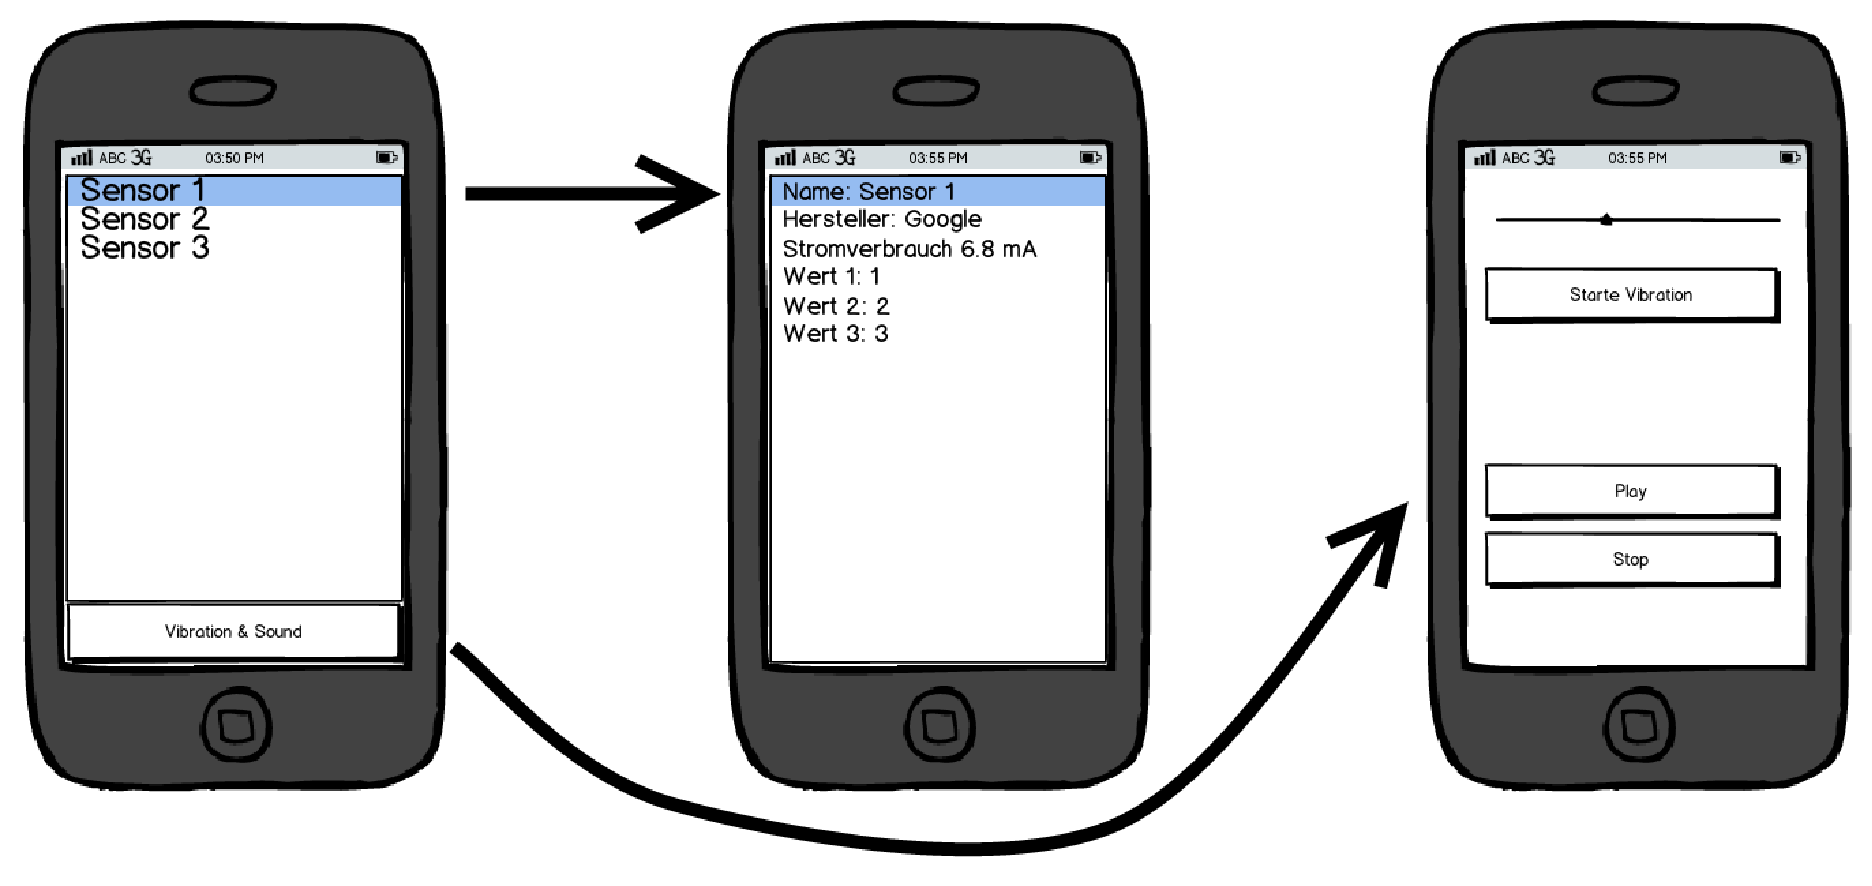
\includegraphics[width=\columnwidth]{example}
    \lfig{example}
    \vspace{-5mm} % use negative white space to fix too large gaps
	\caption{Only include useful figures. Do not simply copy something from a Web.}
\end{figure}



\section{Requirements}
Describe system setup, components, external libraries, hardware etc.


\begin{figure}[h]
	\centering
    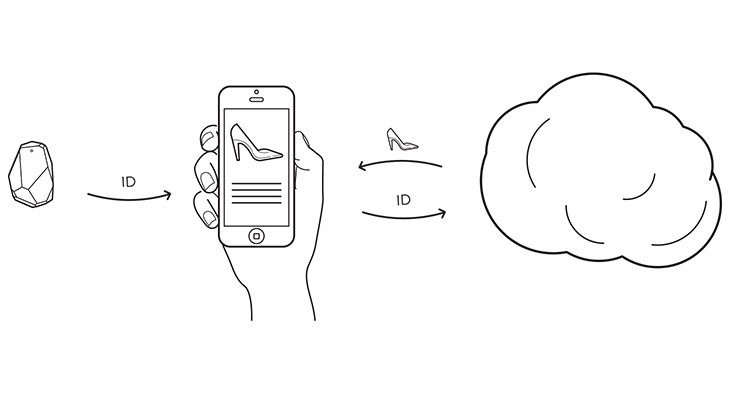
\includegraphics[width=\columnwidth]{overview.jpg}
    \lfig{system-overview}
    \vspace{-5mm} % use negative white space to fix too large gaps
	\caption{System Overview~\cite{estimote}}
\end{figure}

\section{Work Packages}
Breakdown the work to subtasks to meet the project requirements.
Define and describe these tasks.

\begin{itemize}
        \item {\bf WP1}:  XYZ  \ldots    
        \item {\bf WP2}: Set and Configuring Backend Serve  \ldots    
        \item {\bf WP3}: Integration  \ldots 
         \item {\bf WPx}:  \ldots 
\end{itemize}
 
Stick to a concise, scientific writing style. 

\section{Milestones}
The milestones section provides a work plan for carrying out the project.
This is your schedule for getting the project done.
Clearly state how the work packages will be distributed among the team members. 
% The following two commands are all you need in the
% initial runs of your .tex file to
% produce the bibliography for the citations in your paper.
\bibliographystyle{abbrv}
\bibliography{report}  % sigproc.bib is the name of the Bibliography in this case
% You must have a proper ".bib" file

%\balancecolumns % GM June 2007

\end{document}
